\chapter[k-means approach]{\textit{k}-means approach for cluster analysis}
This chapter illustrates the implementations of the $k$-mean algorithm on a matrix of general practitioners and prescriptions for antibiotic, to classify them according to their behaviour.

\textbf{\textit{k}-means clustering} is the most commonly used unsupervised machine learning algorithm for dividing a given dataset into $k$ clusters. 

This method related to antibiotic resistance research consists in applying a time series clustering approach to \textit{group general practitioners according to their prescriptive habits of antibiotics}, using medicines as profiling instrument to obtain models of usage for each product.

Additional layers (factors) to consider while profiling are space, time, structure and personal information of patients, to highlight potential behaviours to classify doctors and co-prescription activities. 

Data has therefore to be subject of parsing, grouping values b to chosen features and selecting subsets based on consistency, maximising potential given information. 

Records will be mapped into a $n$-dimensional matrix which will be fed to the algorithm, obtaining a cluster of belonging for each element. Dimensions will represent \textbf{individuals}, \textbf{relevant features} and \textbf{time}, yet time slices will be taken separately to be able to make comparisons and predictions. 

Results aim to identify whether general practitioners are ``loyal'' prescribers: having most prescribed antibiotics, checking whether there exist typologies of patterns according to active and illustrative variables. 

$k$-means is the chosen clustering algorithm, since the approach is non-hierarchical and simple: its minimum computation complexity and ease of use make it the most suitable algorithm to perform an initial clustering on raw data, reducing the space into disjoint smaller sub-spaces to then perform additional analysis.

After identifying the clusters and linking each one with a specific prescription patten, it is possible to discriminate between GPs with \textit{changing} and \textit{constant} behaviours among time.

\section{Range of time}
Since the aim of clustering is identifying prescription patterns and their changes, extracting \textbf{different time slices} allows better insights on evolutions of trends.

To avoid the impact of seasonality, having values increasing in the winter months, data is collected and aggregated in a range of \textbf{one year}: the final table contains cumulative results and features, without distinction between different times of the year.

Comparisons are made selecting two snapshots of data according to different years, and visualising outcomes to understand whether values have shifted cluster (general practitioners have changed habits).

Data in two years needs to be distant enough to ensure the presence of potential changes, yet consistent enough to prevent information loss. 

Selected years are \textbf{2010} and \textbf{2017}, 2017 being the latest complete time range and 2010 being the first year considered for antibiotics analysis.

\section{Dataset construction}
Before being able to apply a clustering algorithm, data has to be cleaned, arranged and aggregated: having a format of single prescription records would not give the desired outcome, since grouping has to be made according to \textit{counts in years}.

\textbf{Transposing} information from a row to a column visualisation allows to emphasise the values of each feature.

The most important constraint while constructing the matrix is consistency of data: all general practitioners must be active in both years, to make comparison possible.

The number of constantly active doctors is 372, having respectively 228 022 and 214 316 patients in 2010 and 2017. This implies a data loss of about 75\% in both sets.

Features to consider are:
\begin{itemize}
	\item Antibiotic prescriptions;
	\item Patients data;
	\item Other prescriptions' habits data.
\end{itemize}

To limit horizontal expansion of the matrix, a limited number of attributes are taken into account, chosen by their relevancy:
\begin{itemize}
	\item Antibiotic prescriptions are broken and counting according to the \textbf{8 most popular products} (Augmentin, Normix, Ciproxin, Levoxacin, Monuril, Velamox, Rocefin, Zitromax);
	\item Patients data only includes \textbf{gender} and most common \textbf{age range} in $\{1, 2, 3, 4\}$. 
\end{itemize}

Other prescriptions' data has been limited to the \textit{total number of prescriptions} (not strictly related to antibiotics) for each year. Information about the total amount of prescriptions might be helpful to understand the percentage of antibiotics respecting to the whole, and therefore their influence.

According to the goal of the analysis, every sample is represented as a \textbf{13-dimensional vector}, with each row containing information on a single general practitioner.

Displayed below is an extract of the final table for 2017:
\begin{center}
	\begin{table}[h]
	 \makebox[\textwidth][c]{
	\begin{tabular}{c|c|c|c|c|c|c|c|c}
		\textbf{\#} & \textbf{Doctor ID} & \textbf{Aug.} & \textbf{Normix} & \dots & \textbf{M. patients} & \textbf{F. patients} & \textbf{Age} & \textbf{Prescriptions} \\
		\hline
		1 & DRTQRGJ & 5 & 123 & \dots & 303 & 397 & 3 & 17 862 \\
		\hline 2 & DSJRY7B & 242 & 131 & \dots & 322 & 399 & 4 & 15 845 \\
	\end{tabular}}
\caption{\small $k$-means matrix extract}
\vspace{-20px}
\end{table}
\end{center}

Input matrix has dimensions of $372 \times 13 \times 2$, where the latter is an additional time dimension which distinguishes between 2000 and 2017, removed splitting the dataset to run the algorithm separately in the two years.

\section{Features selection}
Having too many features, despite the initial grouping, may lead to overfitting and having general practitioners clustered according to irrelevant information.

Among all features, some are relevant for the outcome of the algorithm, while others are purely descriptive to be checked after clustering results.

All the amounts of \textit{prescriptions} for each antibiotic (columns 1-9) have to be considered to extract similarity, and scaled to normalise numbers. Those count as \textbf{active variables}, and clustering will be performed considering the subset of belonging.

Doctors' IDs are removed during computation, to then be added back to map each row with its belonging individual. 

The other attributes are \textbf{illustrative}, and will be attached to clustering results, to offer further information to be compared after having a general idea of each doctor's group. 

\section{Optimal number of clusters}
Determining the most suitable number of clusters in a data set is a fundamental issue in $k$-means clustering, which requires the user to specify the number of clusters $k$ to be generated. There are various approaches to pick the best value, yet the method is ultimately subjective\cite{silhouette}.

\subsection{\texttt{NbClust}}
\texttt{NbClust} is a R package which provides 30 indices for determining the number of clusters and proposes the best clustering scheme from the different results obtained by varying all combinations of number of clusters, distance measures, and clustering methods. 

Both datasets have been tested with \texttt{NbClust} using number of clusters in $\{2, 20\}$.

Results for 2010:
\begin{lstlisting}
* Among all indices:                                                
* 8 proposed 2 as the best number of clusters 
* 2 proposed 3 as the best number of clusters 
* 1 proposed 7 as the best number of clusters 
* 7 proposed 8 as the best number of clusters 
* 1 proposed 12 as the best number of clusters 
* 1 proposed 14 as the best number of clusters 
* 2 proposed 15 as the best number of clusters 
* 1 proposed 20 as the best number of clusters 

***** Conclusion *****                            

* According to the majority rule, the best number of clusters is  2 
\end{lstlisting}

Results for 2017:
\begin{lstlisting}
* Among all indices:                                                
* 9 proposed 2 as the best number of clusters 
* 1 proposed 3 as the best number of clusters 
* 1 proposed 6 as the best number of clusters 
* 3 proposed 9 as the best number of clusters 
* 1 proposed 14 as the best number of clusters 
* 1 proposed 15 as the best number of clusters 
* 1 proposed 18 as the best number of clusters 
* 2 proposed 19 as the best number of clusters 
* 5 proposed 20 as the best number of clusters 

***** Conclusion *****                            

* According to the majority rule, the best number of clusters is  2 
\end{lstlisting}

It can be seen that indices give 2 as optimal number of clusters for both matrices.

\subsection{Elbow and silhouette}
Direct methods consist in optimizing a criterion, such as the within cluster sums of squares or the average silhouette. The corresponding methods are named elbow and silhouette methods, respectively.

A detailed trend on the optimal number of clusters can be obtained applying respectively the WSS (Within Sum of Squares) and silhouette indexes in R.

The basic idea behind partitioning methods is to define clusters such that the total intra-cluster variation (or total within-cluster sum of square, WSS) is minimized. The total WSS measures the compactness of the clustering, which should be as small as possible.

The Elbow method looks at the total WSS as a function of the number of clusters: one should choose a number of clusters so that adding another cluster doesn't improve much better the total WSS.

Average silhouette method computes the average silhouette of observations: it measures how similar a sample is to the others belonging to the same cluster, compared to how similar it is to the others in different clusters, estimating the distance between clusters for different values of $k$.

The optimal number of clusters $k$ is the one that maximize the average silhouette over a range of possible values\cite{silhouette}.

\begin{figure}[h]
	\centering
	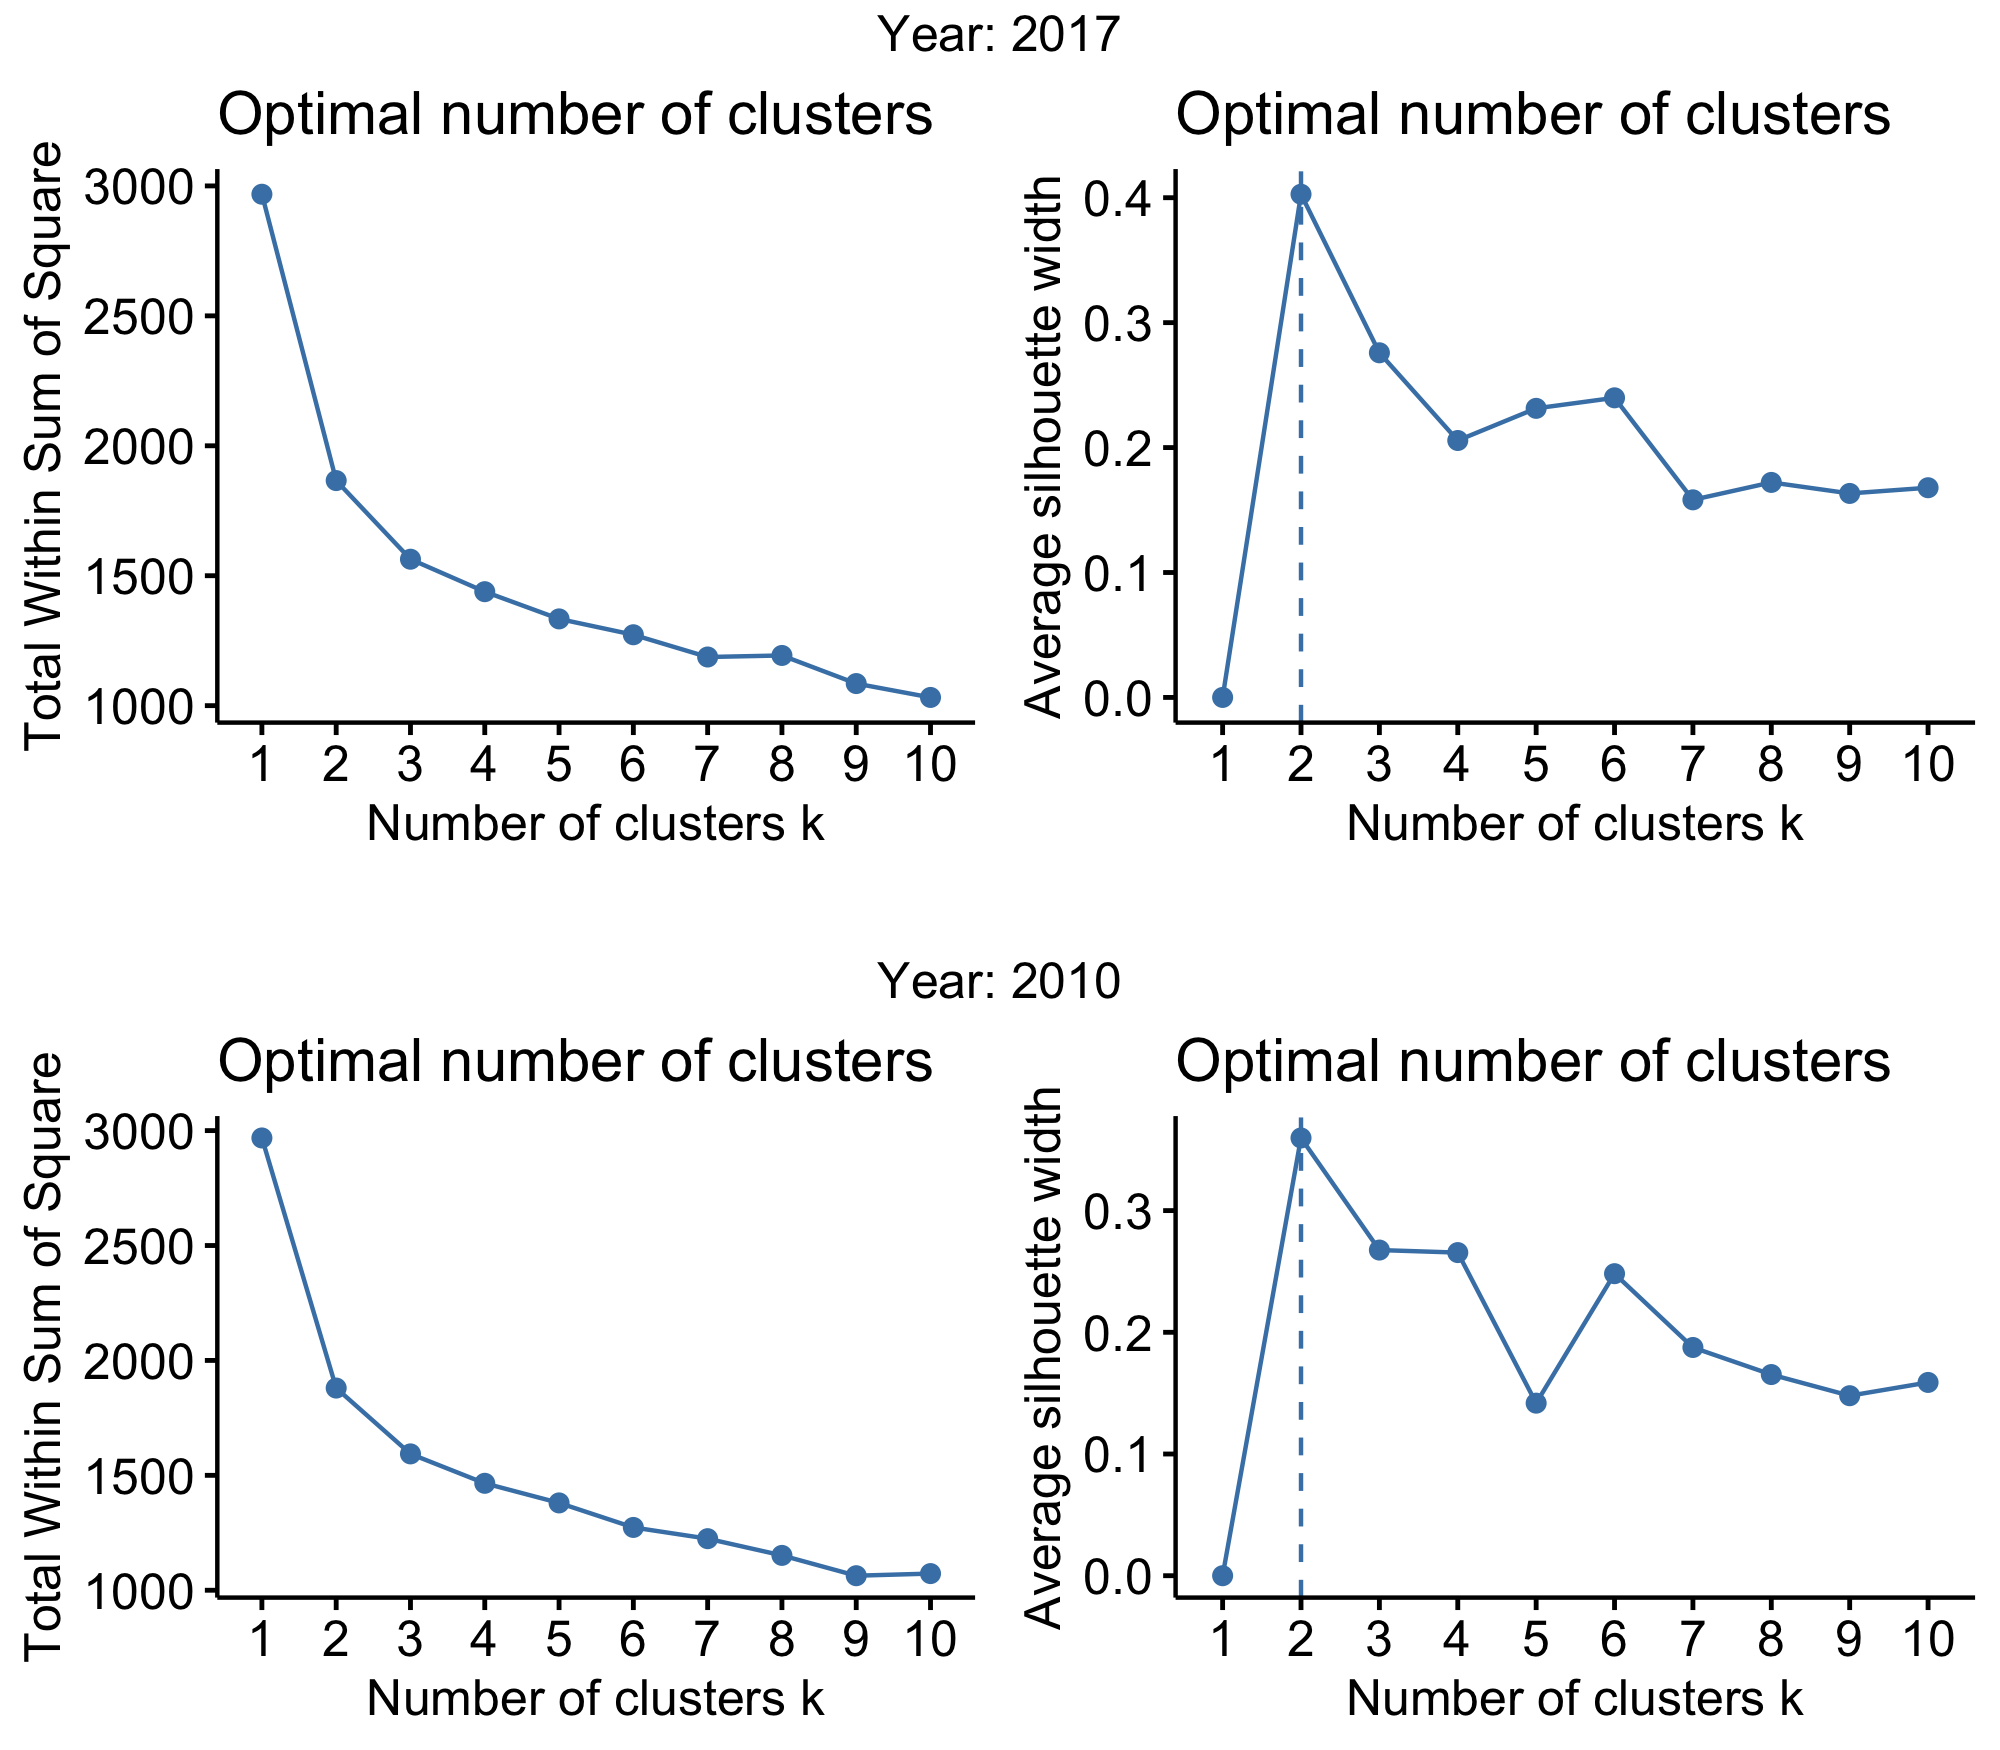
\includegraphics[scale=0.22]{../k-means/optimal-clusters.png}
	\caption{\small WSS and silhouette indexes for $k$-means}
\end{figure}

It can be seen in the figure that both indexes show 2 as the best number, coherently with \texttt{NbClust}, yet 5 or 6 clusters give an acceptable score as well.

Having 2 clusters increases the risk of classification according to \textbf{irrelevant features}, such as large and small prescribers, giving no other useful information.

Therefore, the algorithm is subject of an \textbf{additional run} with an arbitrary amount of 4 clusters, observing how many individuals compose each cluster and eventually adjusting the value of $k$.

\section{Results}

\subsection{2 clusters} 

\subsubsection{Year 2010}
\begin{center}
	\begin{table}[h]
	\makebox[\textwidth][c]{
		\begin{tabular}{c|c|c|c|c|c|c|c|c|c}
			\textbf{\#} & \textbf{Augmentin} & \textbf{Normix} & \textbf{Ciproxin} & \textbf{Levox.} & \textbf{Mon.} & \textbf{Vel.} & \textbf{Roc.} & \textbf{Zitr.} & \textbf{Size} \\
			\hline
			1 & 64,44 & 52,95 & 36,96 & 37,39 & 32,23 & 34,45 & 25,88 & 25,15 & 232 \\
			\hline
			2 & 224,59 & 131,29 & 86,29 & 80,10 & 80,25 & 99,74 & 62,08 & 54,15 & 140 \\
	\end{tabular}}
\caption{\small $k$-means with 2 clusters, 2010}
\vspace{-30px}
\end{table}
\end{center}
\medskip

\subsubsection{Year 2017}
\begin{center}
	\begin{table}[h]
	\makebox[\textwidth][c]{
		\begin{tabular}{c|c|c|c|c|c|c|c|c|c}
			\textbf{\#} & \textbf{Augmentin} & \textbf{Normix} & \textbf{Ciproxin} & \textbf{Levox.} & \textbf{Mon.} & \textbf{Vel.} & \textbf{Roc.} & \textbf{Zitr.} & \textbf{Size} \\
			\hline
			1 & 95,69 & 70,46 & 49,27 & 42,37 & 37,51 & 21,74 & 36,17 & 32,14 & 242 \\
			\hline
			2 & 316,50 & 185,61 & 104,90 & 86,72 & 89,07 & 42,25 & 77,11 & 79,42 & 130 \\
	\end{tabular}}
\caption{\small $k$-means with 2 clusters, 2017}
\vspace{-30px}
\end{table}
\end{center}
\medskip

\subsubsection{Considerations}
The two clusters have a consistent different between the \textbf{means} of antibiotic prescriptions' amounts, especially Augmentin and Velamox, which are the most popular. 

This leads to considering two clusters as \textit{heavy} prescribers and \textit{light} ones, as expected.

Comparison between total prescriptions of members of each cluster:
\begin{table}[h]
	\centering
	\begin{tabular}{c|c|c|c}
		\textbf{Year} & \textbf{Cluster} & \textbf{Mean} & \textbf{SD} \\
		\hline
		2010 & 1 & 9 043,41 & 5 120,81 \\
		\hline
		2010 & 2 & 18 228,35 & 5 314,28 \\
		\hline
		2017 & 1 & 10 126,52 & 5 392,88 \\
		\hline
		2017 & 2 & 19 755,14 & 5 360,95 \\
	\end{tabular}
\caption{\small Comparison of total prescriptions within clusters}
\end{table}

Standard deviation of total amount of prescription is overall the same, which implies clustering has consistent and related results. Mean between first and second cluster tends to increase during the years, yet is still close.

This confirms the hypothesis of grouping according to the number of prescriptions.

The amount of general practitioners in the clusters is almost the same from 2010 to 2017, with 78 doctors swapping clusters in total:
\begin{itemize}
	\item 44 switched from large prescribers to small ones;
	\item 34 switched from small prescribers to large ones.
\end{itemize}
The difference of 10 switching doctors is the same as the difference between cluster 1 in 2010 and cluster 1 in 2017.

General practitioners overall remained mostly stable with their amount of prescriptions, yet some switched habits while the mean of total prescriptions increased. This most likely implies that doctors classified as large prescribers still consistently increased their numbers, so that the mean grew by roughly 1 000 in 7 years, although some doctors started to prescribe less.

Clusters for each year are shown performing a PCA among the considered features (number of prescriptions for each antibiotic) with the \texttt{fviz\_cluster} function from package \texttt{factoextra}. 

\begin{figure}[h]
	\centering
	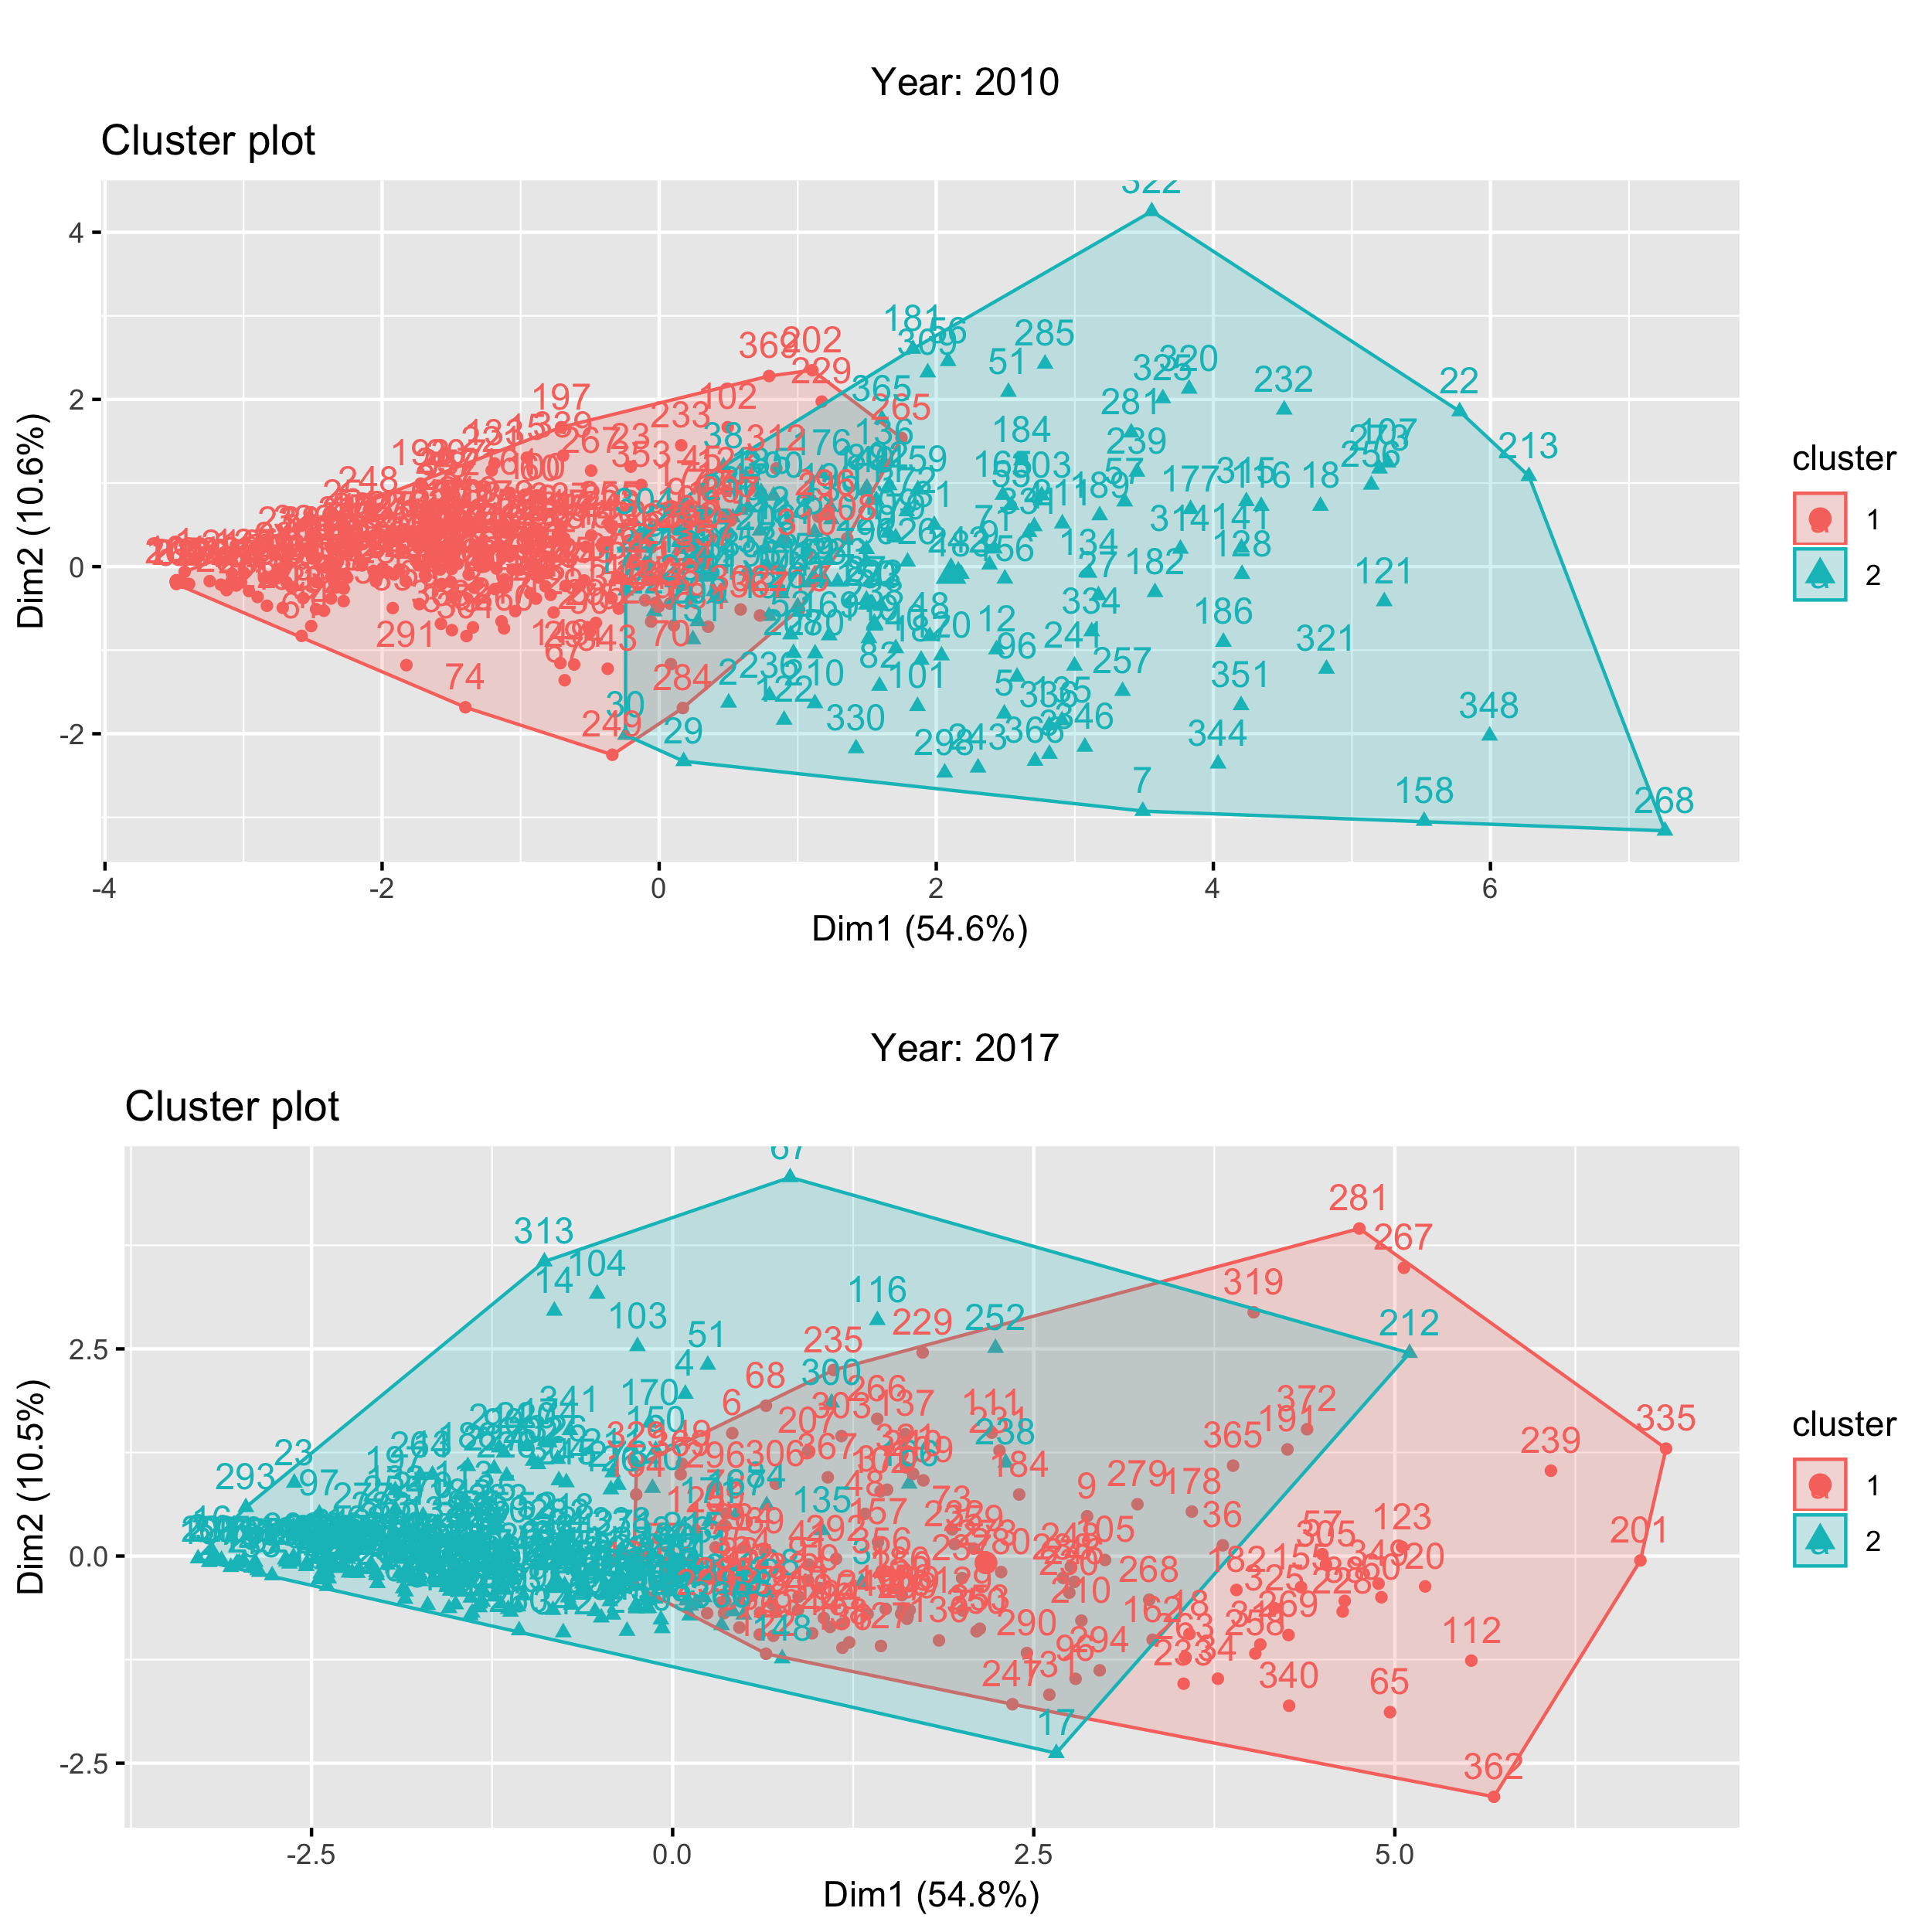
\includegraphics[scale=0.18]{../k-means/clusters-2.png}
	\caption{\small PCA with 2 clusters}
\end{figure}

Each number represents the row corresponding to a general practitioner, while the axes are principal components. Clusters tend to overlap because of the dimensionality reduction.

\subsection{4 clusters}

\subsubsection{Year 2010}
\begin{center}
	\begin{table}[h]
 \makebox[\textwidth][c]{
		\begin{tabular}{c|c|c|c|c|c|c|c|c|c}
			\textbf{\#} & \textbf{Augmentin} & \textbf{Normix} & \textbf{Ciproxin} & \textbf{Levox.} & \textbf{Mon.} & \textbf{Vel.} & \textbf{Roc.} & \textbf{Zitr.} & \textbf{Size} \\
			\hline
			1 & 291,35 & 187,93 & 107,84 & 94,42 & 102,02 & 159,28 & 70,68 & 65,37 & 45 \\
			\hline
			2 & 86,85 & 120,96 & 68,14 & 70,03 & 65,63 & 76,75 & 48,13 & 47,63 & 61 \\
			\hline
			3 & 195,29 & 85,38 & 69,41 & 61,93 & 61,60 & 57,77 & 50,10 & 43,20 & 103 \\
			\hline
			4 & 48,27 & 37,02 & 27,59 & 30,61 & 23,15 & 25,51 & 20,97 & 19,14 & 163 \\
	\end{tabular}}
\caption{\small $k$-means with 4 clusters, 2010}
\vspace{-30px}
\end{table}
\end{center}
\medskip

\subsubsection{Year 2017}
\begin{center}
	\begin{table}[h]
	\makebox[\textwidth][c]{
		\begin{tabular}{c|c|c|c|c|c|c|c|c|c}
			\textbf{\#} & \textbf{Augmentin} & \textbf{Normix} & \textbf{Ciproxin} & \textbf{Levox.} & \textbf{Mon.} & \textbf{Vel.} & \textbf{Roc.} & \textbf{Zitr.} & \textbf{Size} \\
			\hline
			1 & 397,54 & 236,54 & 124,08 & 101,05 & 107,93 & 55,01 & 87,51 & 112,71 & 59 \\
			\hline
			2 & 32,57 & 165,30 & 89,50 & 90,31 & 76,88 & 47,65 & 72,69 & 69,80  & 26 \\
			\hline
			3 & 228,18 & 119,93 & 78,85 & 63,74 & 63,15 & 28,99 & 59,01 & 46,01 & 117 \\
			\hline
			4 & 78,24 & 52,33 & 39,33 & 33,88 & 28,84 & 16,92 & 28,36 & 25,03 & 170 \\
	\end{tabular}}
\caption{\small $k$-means with 4 clusters, 2017}
\vspace{-30px}
\end{table}
\end{center}

\subsubsection{Considerations}
According to the cluster means for each antibiotic, general practitioners within clusters can be classified as:
\begin{enumerate}
	\item Large prescribers;
	\item Strong preference for Normix;
	\item Strong preference for Augmentin;
	\item Small prescribers.
\end{enumerate}

It can be seen that Augmentin means for cluster 3 is higher than the Normix one for cluster 2: Augmentin is most likely the over-prescribed drug.

Similarities in clusters composition:
\begin{itemize}
	\item 28 doctors being large prescribers in 2010 stayed constant in 2017;
	\item 12 doctors being Normix prescribers in 2010 stayed constant in 2017;
	\item 55 doctors being Augmentin prescribers in 2010 stayed constant in 2017;
	\item 122 doctors being small prescribers in 2010 stayed constant in 2017.
\end{itemize}

Similarities show 20-40 doctors for each cluster switching prescription habits, with a total of 155 elements belonging to a different groups. Considering 372 original individuals, this consists in 41,6\%.

Cluster size varies, with cluster 2 being subject of a consistent decrease in the number of elements from 2010 to 2017, while all the others increase size. Normix prescribers, then, switched to another category.

Comparison between total prescriptions of members of each cluster:
\begin{table}[h]
	\centering
	\begin{tabular}{c|c|c|c}
		\textbf{Year} & \textbf{Cluster} & \textbf{Mean} & \textbf{SD} \\
		\hline
		2010 & 1 & 22 244,29 & 4 540,88 \\
		\hline
		2010 & 2 & 15 587,75 & 4 328,30 \\
		\hline
		2010 & 3 & 14 910,14 & 4 574,42 \\
		\hline
		2010 & 4 & 7 131,60 & 4 326,86 \\
		\hline
		2017 & 1 & 23 154,69 & 4 523,31 \\
		\hline
		2017 & 2 & 17 481,92 & 5 370,08 \\
		\hline
		2017 & 3 & 15 042,37 &4 699,17 \\
		\hline
		2017 & 4 & 8 459,83 & 4 601,97 \\
	\end{tabular}
	\caption{\small Comparison of total prescriptions within clusters}
\end{table}

Standard deviation tends to stay constant, and mean for large and small prescribers is widely different, therefore the predictions seem to be correct. Mean between Normix and Augmentin prescribers is similar, meaning that both general practitioners having this behaviour do not tend to overprescribe other medicines.

To have a detailed view of changes between Normix and Augmentin preferences, those groups are compared to each other and the major prescribers cluster:
\begin{itemize}
	\item 26 Normix prescribers in 2010 switched to Augmentin in 2017;
	\item 4 Augmentin prescribers in 2010 switched to Normix in 2017;
	\item 5 Normix prescribers in 2010 switched to large prescribers in 2017;
	\item 22 Augmentin prescribers in 2010 switched to large prescribers in 2017.
\end{itemize}

Normix prescribers progressively switched to large prescribers (cluster 1) or having Augmentin preference (cluster 3), and all Augmentin averages increased: in particular in cluster 1, those have an additional 100 prescriptions in 2017.

It is safe to assume that although small prescribers represent a considerable percentage of the total, Augmentin prescriptions are being pushed upwards, most likely because of antibiotic resistance and general practitioners' tendency to overprescribe.

Performing a run of the algorithm only using Augmentin and Normix values shows that, despite 2010 being the same, Normix prescriptions in 2017 aren't relevant enough to be the main characteristic of a cluster. 

Normix has therefore lost popularity within years: this is confirmed by antibiotics' trends graphs, showing a constant value for Normix prescriptions in the last years while Augmentin has a steady increase.

All the other antibiotics have constant trends as well, aside from the general raise from 2012 to 2015, yet values are consistently smaller, hence why the algorithm does not assess particular importance to them. 

Clusters for each year are again shown performing a PCA with \texttt{fviz\_cluster}.

\begin{figure}[h]
	\centering
	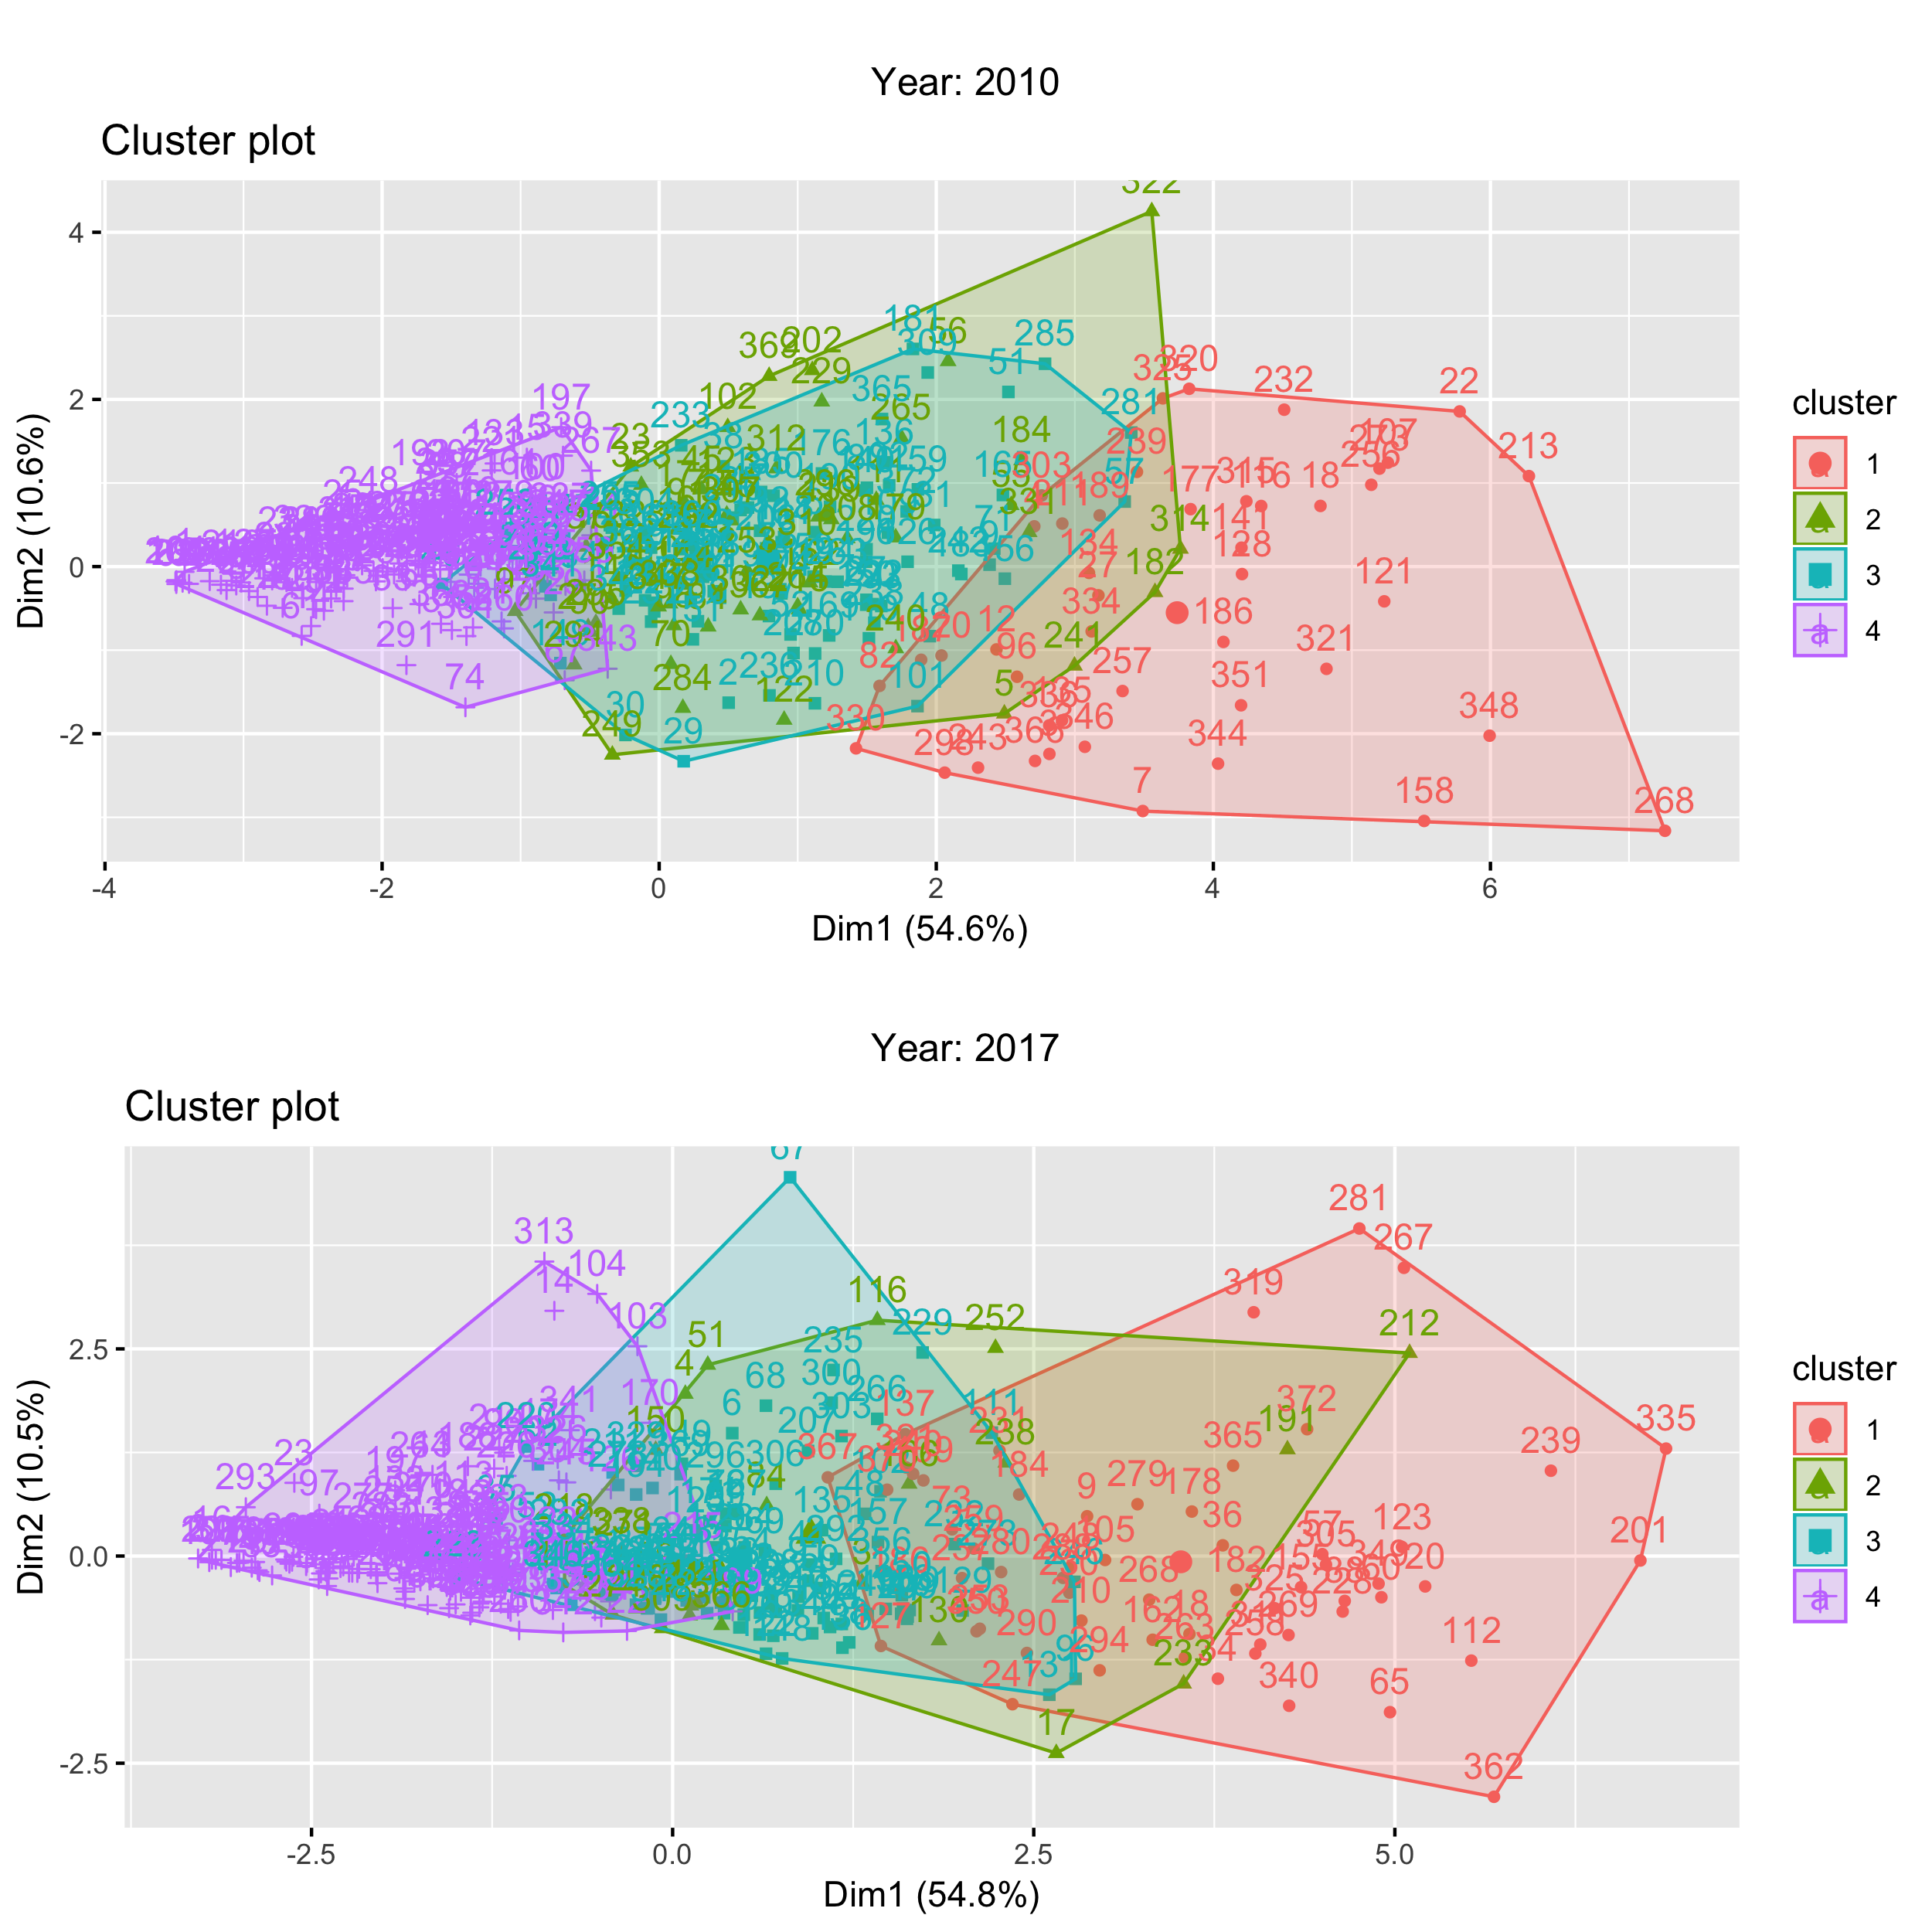
\includegraphics[scale=0.18]{../k-means/clusters-4.png}
	\caption{\small PCA with 4 clusters}
\end{figure}
